\documentclass[12pt,a4paper]{article}
\usepackage[UTF8]{ctex}
\usepackage{amsmath,amssymb}
\usepackage{booktabs}
\usepackage{float}
\usepackage{fancyhdr}   % 页眉页脚控制
\usepackage{geometry}
\usepackage{subfigure}  % 子图排版
\usepackage{subcaption}
\usepackage{graphicx}
\usepackage{listings} % 代码排版宏包
\usepackage{xcolor} % 代码高亮颜色
\usepackage{enumitem} % 列表格式控制宏包
\geometry{left=2.5cm,right=2.5cm,top=2.5cm,bottom=2.5cm}

\pagestyle{fancy}
\fancyhf{} % 清空默认页眉页脚
\fancyhead[L]{\small 直流双臂电桥}       % 左上角页眉
\fancyhead[R]{\small 2513318}          % 右上角章节名
\fancyfoot[C]{\thepage}                   % 居中页码（页脚）
\renewcommand{\headrulewidth}{0.4pt}      % 页眉线粗细
\renewcommand{\footrulewidth}{0.4pt}      % 页脚线粗细
%报告开始
\begin{document}
	%设置课程标题
	\begin{center}
		\heiti\LARGE{《大学基础物理实验》课程实验报告}
	\end{center}
	%设置实验人信息以及实验时间表格
	\begin{center}
		\begin{tabular}{lcr}
			{\songti 姓名及学号：陈秋实2513318}  \quad 专业：密码科学与技术 \quad 组别：L组1号 \\
			{\songti  学院：密码与网络空间安全学院 \quad 实验时间：2026年4月24日~星期五~下午}\\
		\end{tabular}
	\end{center}
	\vspace{-0.2cm}
	{\noindent}	 \rule[-10pt]{16cm}{0.05em}\\
	\vspace{-0.4cm}
	%实验题目
	\begin{center}
		\LARGE\textbf{直流双臂电桥}
	\end{center}
	
	%实验原理
	\section{实验原理}
	\subsubsection*{直流双臂电桥适用范围：}
	\par 直流双臂电桥适用于测量较小的电阻，如QJ44型直流双臂电桥测量范围: 0.1m$\Omega$-11$\Omega$
	\subsubsection*{四端法：}
	\begin{figure}[!htbp]
		\centering
		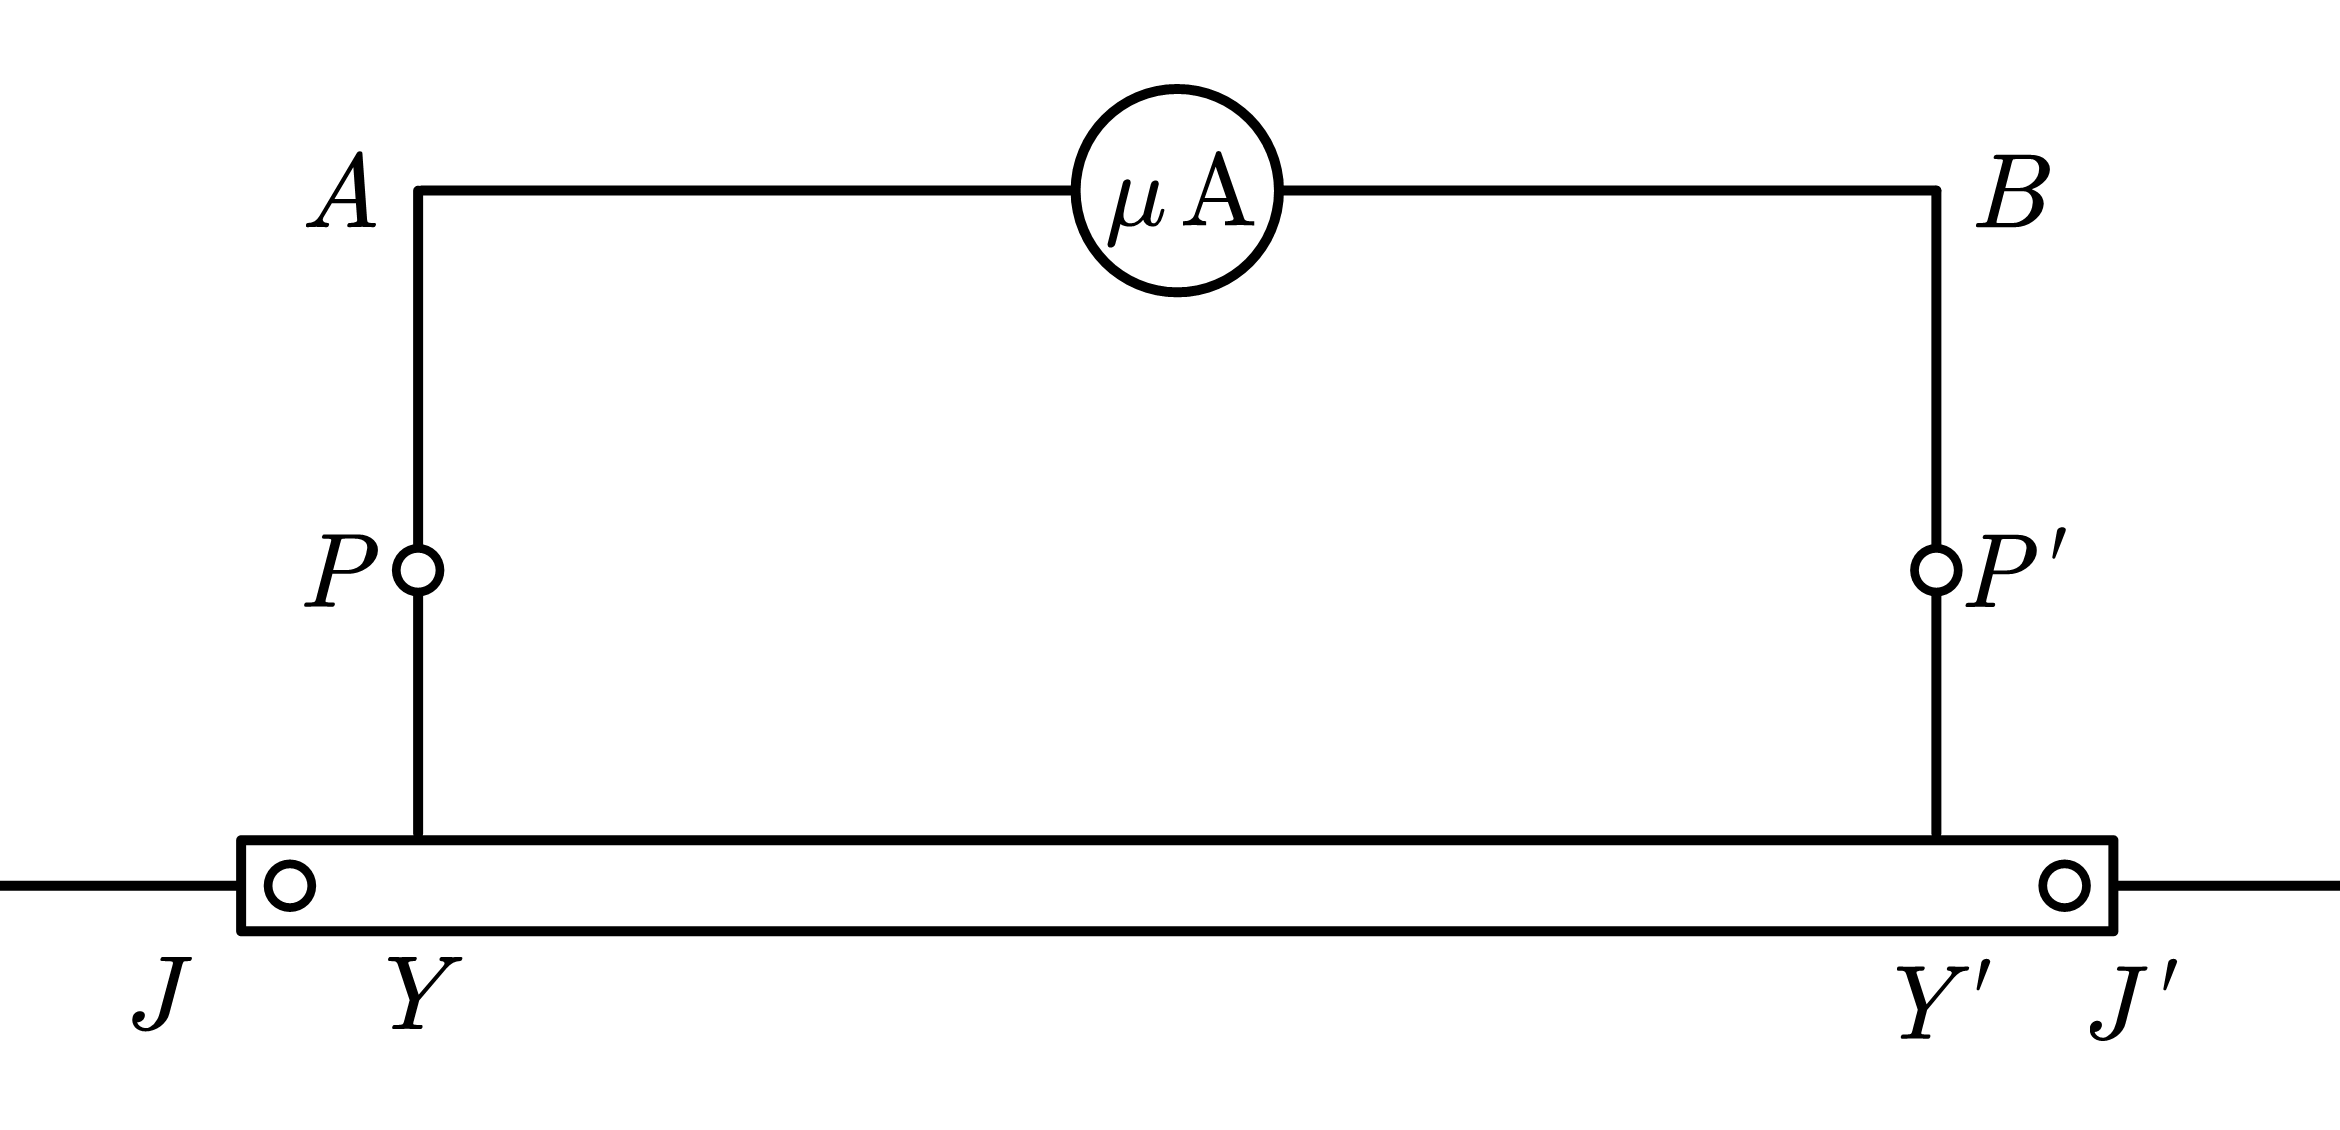
\includegraphics[width=0.6\textwidth]{四端法.png}
		\caption{四端法原理}
	\end{figure}
	\par 可以看出，使用图1的电路进行测量，在电阻体上$Y,Y^{\prime}$上两个点焊出两个接头再与微安表相连接，这样可以保证微安表所连接两点之间的阻值正好为$Y,Y^{\prime}$之间的阻值，又$A,B,P,P^{\prime}$四个点的接触电阻和$AY,BY^{\prime}$的接线电阻都分给了微安表，保证了分流的精确。由于电阻被做成了四个接头，故称作“四端结构”。
	
	\subsubsection*{实验电路与测量公式推导}
	\par 测量电路如图2(见下页)所示，其中$R_0$为标准低阻，$R_x$为待测低阻。四个比例臂电阻有意做成几十欧姆以上的阻值，因此他们所在桥臂中的接线电阻和接触电阻的影响便可忽略。注意右边的电阻$R$是为了防止电流过大。当电流计指零时，电桥达到平衡。
	\clearpage
	\begin{figure}
		\centering
		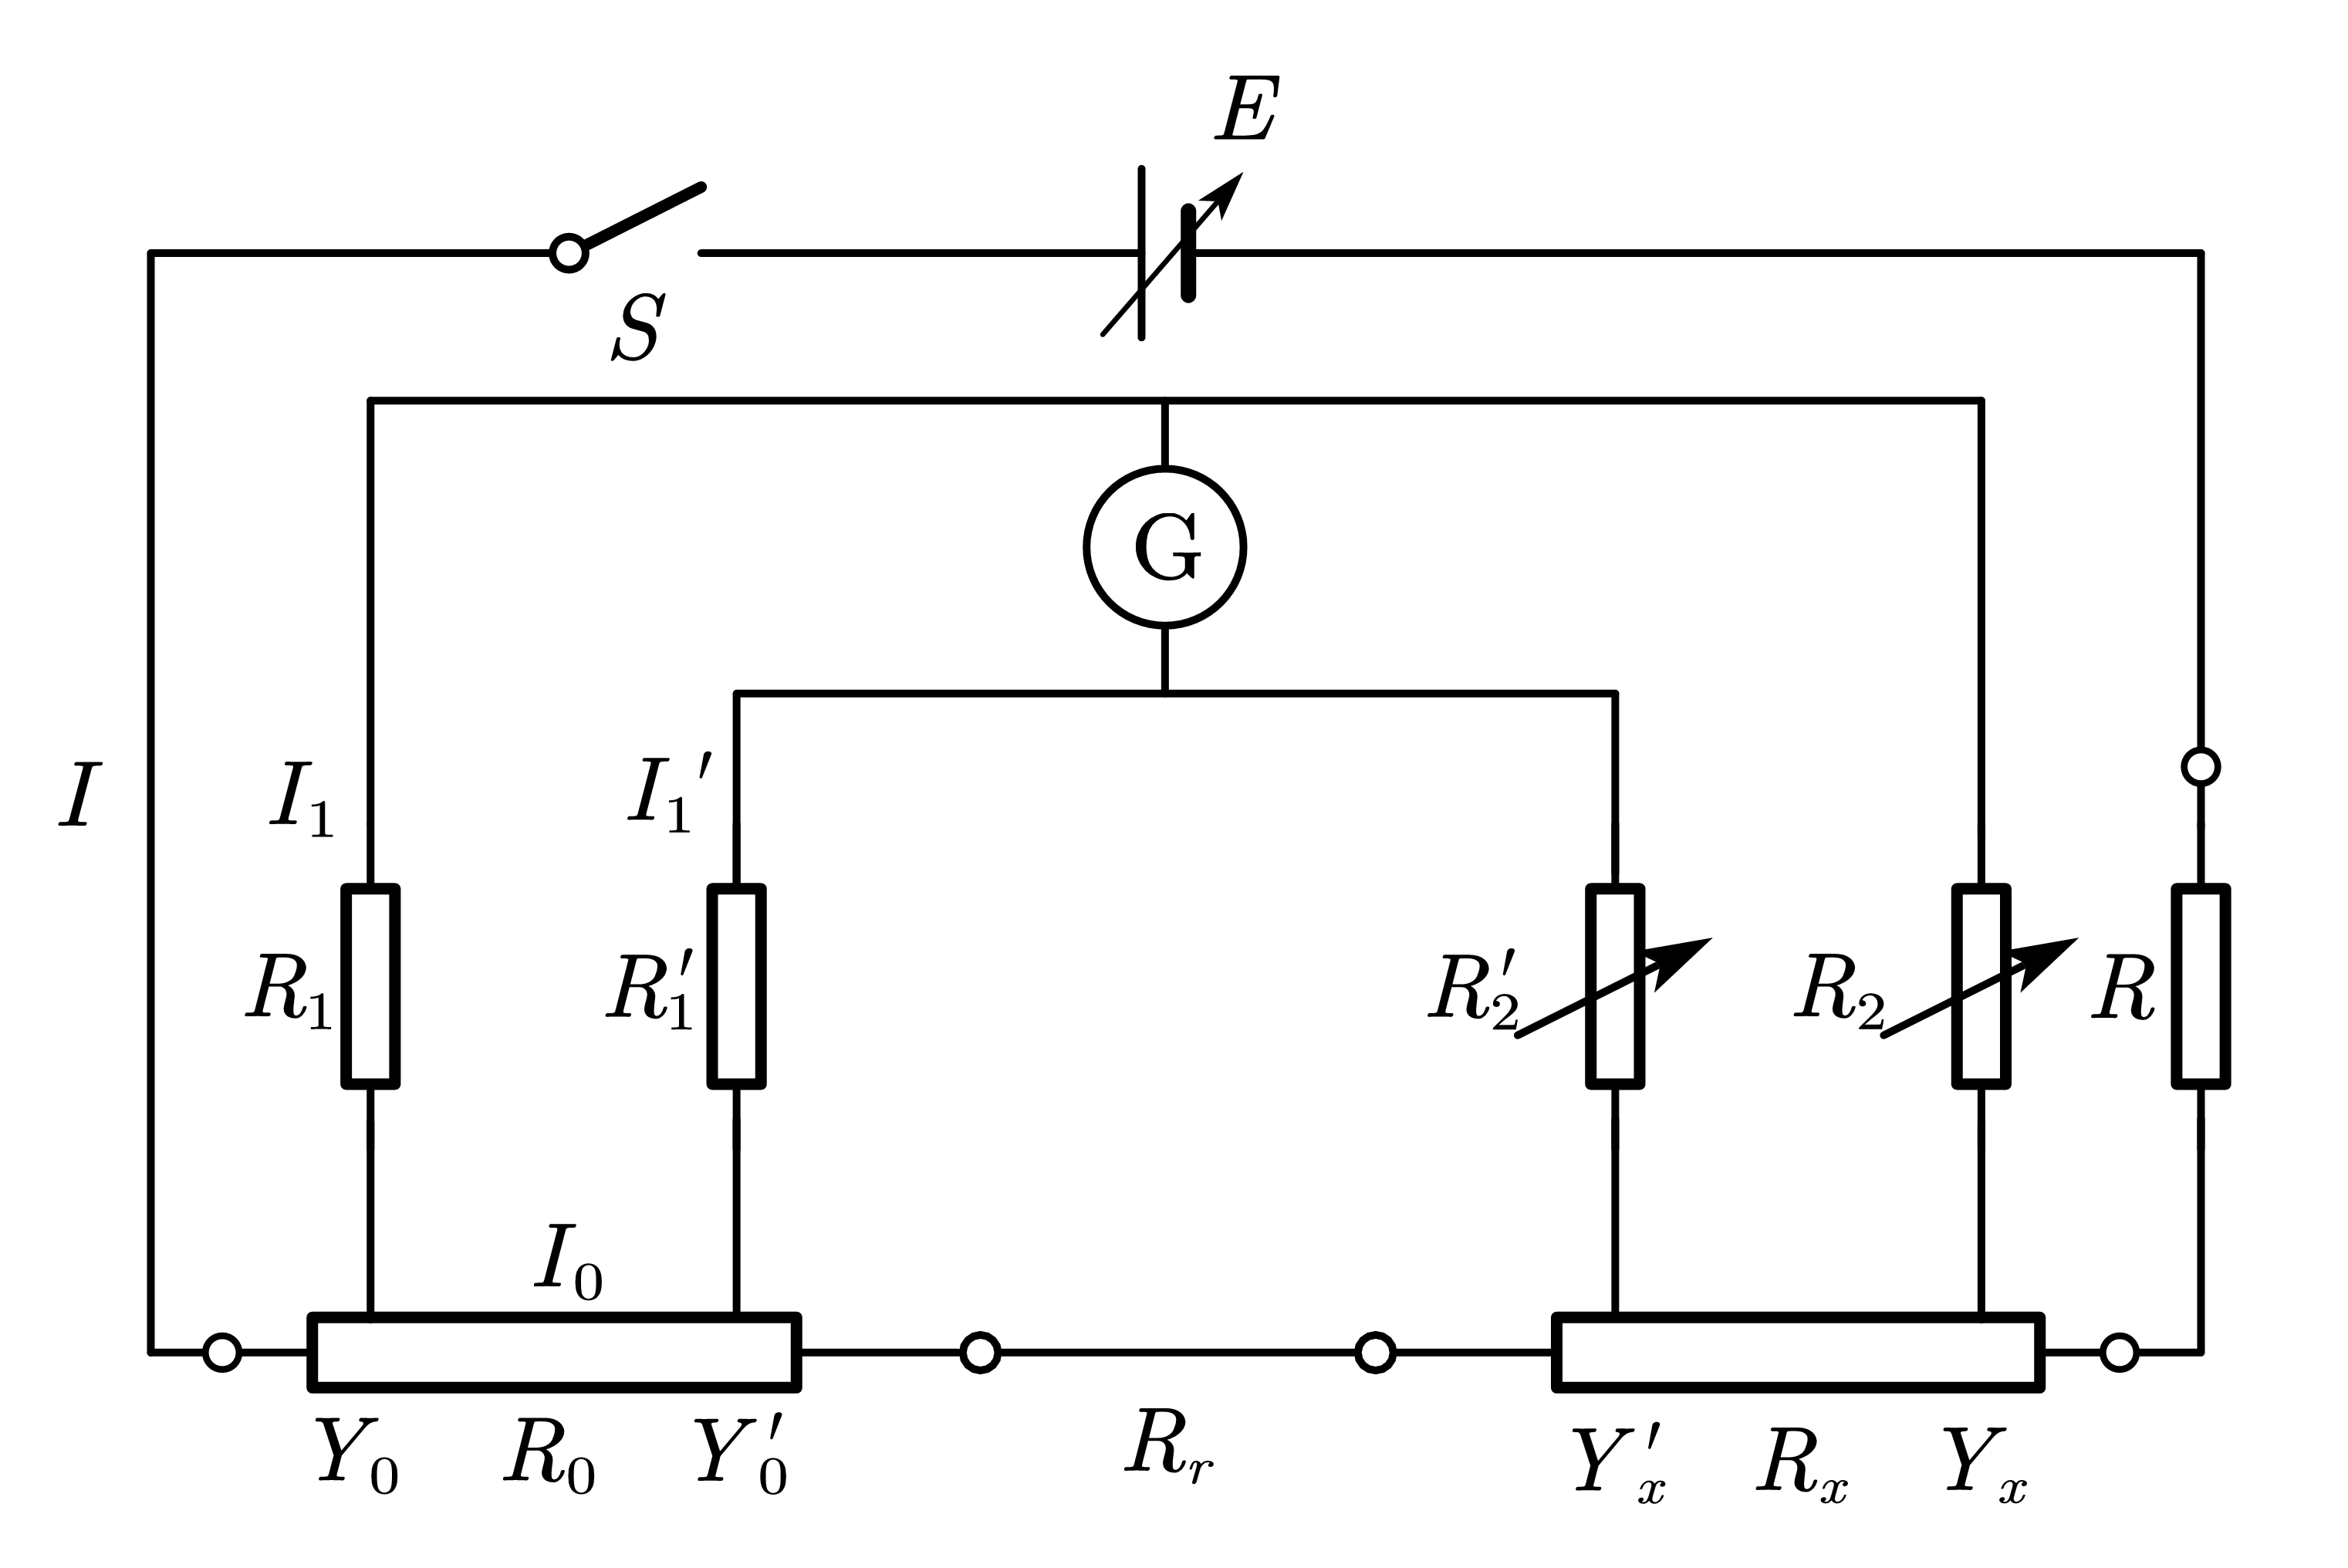
\includegraphics[width=0.6\textwidth]{直流双臂电路图透明.png}
		\caption{直流双臂电路}
	\end{figure}
	\par 由基尔霍夫定律，可以列出方程组：
	
	\begin{equation}
		\begin{cases}
			$$I_1 R_1=I_0 R_0+I_1^{\prime} R_1^{\prime} \\
			I_1 R_2=I_0 R_x+I_1^{\prime} R_2^{\prime} \\
			\left(I_0-I_1^{\prime}\right) R_{\mathrm{r}}=I_1^{\prime}\left(R_1^{\prime}+R_2^{\prime}\right)$$
		\end{cases}
	\end{equation}
	\par 式中$I_1,I_0,I_1^{\prime}$分别为图中所标示，将(1)式整理得：
	\[R_{1}R_{x}=R_{2}R_{0}+(\,R_{2}R_{1}^{\prime}-R_{1}R_{2}^{\prime}\,)\,{\frac{r}{R_{r}+R_{1}^{\prime}+R_{2}^{\prime}}}\]
	\par 当电桥的平衡是在保证$R_{2}R_{1}^{\prime}-R_{1}R_{2}^{\prime}=0$的情况下，则上式可以简化为
	\[R_{x}={\frac{R_{2}}{R_{1}}}R_{0}\]
	\par 由此可知此次实验双臂电桥的测量平衡条件为:
	\[{\frac{R_{2}}{{R_{1}}}}={\frac{{R_{2}^{\prime}}}{{R_{1}^{\prime}}}}={\frac{{R_{x}}}{{R_{0}}}}\]
	\par 本次实验使用同步调节比例臂电阻$R_2,R_2^{\prime}$的方法使电流计示零。
	\subsubsection*{双臂电桥灵敏度}
	\par 双臂电桥平衡后将比例臂电阻$R_2,R_2^{\prime}$同步调偏$\Delta R_2=\Delta R_2^{\prime}$,若电流计示数改变$\Delta I$,则灵敏度$S$为：
	\[
	S=\frac{\Delta I}{\Delta R_2 / R_2}
	\]
	\clearpage
	\par 由$S={\dfrac{\Delta I}{\Delta R_{2}/R_{2}}}={\dfrac{\Delta I}{\Delta R_{x}/R_{x}}}$可以引入相对误差：
	$${\frac{\Delta R_{x}}{R_{x}}}={\frac{\Delta I}{S}}$$
	
	
	\section{数据处理}
	\subsection{数据记录}
	
	\begin{table}[!htbp]
		\centering
		\caption{样品长度测量}
		\begin{tabular}{cc}
			\toprule
			\makebox[0.15\textwidth][c]{样品}&\makebox[0.15\textwidth][c]{长度L(cm)}\\
			\midrule
			铜 & 39.78\\
			铁 & 39.78\\
			铝 & 39.78\\
			\bottomrule
		\end{tabular}
	\end{table}
	
	\begin{table}[!htbp]
		\centering
		\caption{样品直径测量}
		\begin{tabular}{ccccccc}
			\toprule
			\makebox[0.1\textwidth][c]{样品(mm)}&\makebox[0.1\textwidth][c]{测量1}&\makebox[0.1\textwidth][c]{测量2}&\makebox[0.1\textwidth][c]{测量3}&\makebox[0.1\textwidth][c]{测量4}&\makebox[0.1\textwidth][c]{测量5}&\makebox[0.15\textwidth][c]{平均}\\
			\midrule
			铁 & 5.482 & 5.485  & 5.489 & 5.489 & 5.486 &  5.486\\
			铜 & 5.468 & 5.467  & 5.471 & 5.478 & 5.476 &  5.472\\
			铝 & 5.443 & 5.447  & 5.446 & 5.445 & 5.449 &  5.446\\
			\bottomrule
		\end{tabular}
	\end{table}
	
	\begin{table}[!htbp]
		\centering
		\caption{样品阻值测量}
		\begin{tabular}{c|ccc}
			\toprule
			\makebox[0.05\textwidth][c]{X}&\makebox[0.25\textwidth][c]{平衡时:$R_2=R_2^{\prime}(\Omega)$}&\makebox[0.25\textwidth][c]{改变:$\Delta R_2=\Delta R_2^{\prime}(\Omega)$}&\makebox[0.25\textwidth][c]{电流变化:$\Delta I(nA)$}\\
			\midrule
			铁 & 14510 & 200  & 2.7 \\
			铜 & 362.0 & 20   & 3.7 \\
			铝 & 901.2 & 40   & 5.9\\
			\bottomrule
		\end{tabular}
	\end{table}
	
	
	\subsection{样品长度}
	由于是单次测量，故只有B类不确定度，假设误差服从均匀分布，已知米尺的允差$\Delta _x$为0.5mm可知：
	\[
	u_l=u_{Bl}=\frac{\Delta_l}{3}=0.167(mm)
	\]
	\[E_l = \dfrac{u_l}{l}=\left\{
	\begin{aligned}
		&0.042\%\qquad(Cu)\\ 
		&0.042\%\qquad(Fe)\\
		&0.042\%\qquad(Al)\\
	\end{aligned}
	\right.\]
	
	\par 由此可知:三种金属的长度和不确定度分别为
	\begin{table}[!htbp]
		\centering
		\caption{样品长度计算}
		\begin{tabular}{ccc}
			\toprule
			\makebox[0.1\textwidth][c]{样品}&\makebox[0.15\textwidth][c]{长度L(cm)}&\makebox[0.15\textwidth][c]{不确定度(\%)}\\
			\midrule
			铁 & $39.78\pm0.0167$&0.042\\
			铜 & $39.78\pm0.0167$&0.042\\
			铝 & $39.78\pm0.0167$&0.042\\
			\bottomrule
		\end{tabular}
	\end{table}
	  
	  
	\subsection{样品直径}
	已知：$n=5$（测量次数），螺旋测微器分辨率 $\varepsilon_x=0.001\,\text{mm}$ \par
	A类不确定度 \[u_{ax}= \sqrt{\frac{\sum (x_i - \bar{x})^2}{n(n-1)}}\] \par
	B类不确定度 \[
	u_{bx} = \frac{\varepsilon_x}{\sqrt{3}} = \frac{0.001}{\sqrt{3}} \text{mm} = 0.0005\,\text{mm}\] \par
	总不确定度 \[
	u_d = \sqrt{u_{ax}^2 + u_{bx}^2}\]
	
	代入得A类不确定度为：
	\[
	u_{Ad} 
	=\left\{\begin{aligned}
		& 0.0013\qquad(Fe)\\
		& 0.0022\qquad(Cu)\\
		& 0.0010\qquad(Al)
	\end{aligned}\right. \qquad(mm)
	\]
	\par 
	\[
	u_{Bd}=\frac{\varepsilon_d}{\sqrt{3}}=0.0005(mm)
	\]
	\par 从而合成两类不确定度:
	\[
	u_d = \sqrt{u_{Ad}^2+u_{Bd}^2} = \left\{\begin{aligned}
		& 0.0015\qquad(Fe)\\
		& 0.0023\qquad(Cu)\\
		& 0.0012\qquad(Al)
	\end{aligned}\right. \qquad(mm)
	\]
	\[
	E_d = \dfrac{u_d}{d}=\left\{
	\begin{aligned}
		&0.027\%\qquad(Fe)\\ 
		&0.042\%\qquad(Cu)\\
		&0.022\%\qquad(Al)\\
	\end{aligned}
	\right.
	\]
	得到：
	\begin{table}[!htbp]
		\centering
		\caption{样品直径计算}
		\begin{tabular}{ccc}
			\toprule
			\makebox[0.1\textwidth][c]{样品}&\makebox[0.15\textwidth][c]{直径D(mm)}&\makebox[0.15\textwidth][c]{不确定度(\%)}\\
			\midrule
			铜 & $5.486\pm 0.015$&0.027\\
			铁 & $5.472\pm 0.023$&0.042\\
			铝 & $5.446\pm 0.012$&0.022\\
			\bottomrule
		\end{tabular}
	\end{table}
	
	\subsection{$R_x$的测量}
	给定$R_0=0.001\Omega,R_1=1000\Omega$
	\[R_{\overline{x}}={\frac{R_{2}}{R_{1}}}R_{0}=\left\{
	\begin{aligned}
		&0.0145\qquad(Fe)\\ 
		&0.0004\qquad(Cu)\\
		&0.0009\qquad(Al)\\
	\end{aligned}
	\right. \]
	\par 则不确定度为：
	$$
	\rho_x=\left[(1+k)^2\left(\rho_2^2+\rho_1^2\right)+k^2\left(\rho_2^{\prime 2}+\rho_1^{\prime 2}\right)+\rho_0^2+\left(\frac{\delta}{S}\right)^2\right]^{\frac{1}{2}}=\left\{
	\begin{aligned}
		&0.00186\qquad(Fe)\\ 
		&0.00186\qquad(Cu)\\
		&0.00186\qquad(Al)\\
	\end{aligned}
	\right. 
	$$
	\par 
	\begin{table}[!htbp]
		\centering
		\caption{样品阻值计算}
		\begin{tabular}{ccc}
			\toprule
			\makebox[0.1\textwidth][c]{样品}&\makebox[0.3\textwidth][c]{阻值$R_X$($\Omega$)}&\makebox[0.15\textwidth][c]{不确定度(\%)}\\
			\midrule
			铁 & $(145.0\pm 0.2697)\cdot 10^{-4}$&0.186\\
			铜 & $(4.0\pm   0.0074)\cdot 10^{-4}$&0.186\\
			铝 & $(9.0\pm   0.0167)\cdot 10^{-4}$&0.186\\
			\bottomrule
		\end{tabular}
	\end{table}
	
	\subsection{电阻率的计算}
	\[
	\rho = \frac{R_xS}{l}=\frac{R_x\pi d^2}{4l}=\left\{
	\begin{aligned}
		&34.46\times 10^{-8}\qquad(Fe)\\ 
		&0.95 \times 10^{-8}\qquad(Cu)\\
		&4.81 \times 10^{-8}\qquad(Al)\\
	\end{aligned}
	\right. 
	\]
	
	\par \textbf{不确定度的计算}
	\[u_{\rho} = \rho \left[ \left( \frac{u_{Rx}}{R} \right)^2 + \left( \frac{2u_d}{d} \right)^2 + \left( \frac{u_l}{L} \right)^2 \right]^{1/2}
	\]
	
	
	\[
	u_{\rho}=\left\{
	\begin{aligned}
		&1.995\times 10^{-9}\qquad(Fe)\\ 
		&8.187\times 10^{-11}\qquad(Cu)\\
		&2.309\times 10^{-10}\qquad(Al)\\
	\end{aligned}
	\right. 
	\]
	所以得到：
	\begin{table}[!htbp]
		\centering
		\caption{样品长度测量}
		\begin{tabular}{cc}
			\toprule
			\makebox[0.15\textwidth][c]{样品}&\makebox[0.3\textwidth][c]{电阻率}\\
			\midrule
			铁 & $(34.46\pm0.1995)\times 10^{-8}$\\
			铜 & $(0.95 \pm0.0082)\times 10^{-8}$\\
			铝 & $(4.81 \pm0.0231)\times 10^{-8}$\\
			\bottomrule
		\end{tabular}
	\end{table}
	
\end{document}